\documentclass[aspectratio=1610,xcolor=dvipsnames]{beamer}
\usecolortheme{SimplePlus}

\usepackage{graphicx}
\usepackage{tikz}
\usepackage{subcaption}

\title{ProxITR migration regression}
\author{Course Staff}

% Beamer loads amsthm implicitly; ltx-talk does not.
\theoremstyle{plain}
\newtheorem{proxresult}{Result}
% Tagged-math replay must retain this legacy operator idiom.
\newcommand{\diag}{\mbox{{\rm diag}}}

% This visual helper is deliberately unused. It must not block preparation.
\newcommand{\ShowPutAtGrid}{%
  
\begin{tikzpicture}
    \draw[step=1cm] (0,0) grid (2,2);
  \end{tikzpicture}%
}

% This is the Beamer overlay-aware form used by the original slide deck.
% The generated ltx-talk compatibility shim must preserve its argument order.
\newcommand<>{\NormalBox}[1]{%
  \only#2{\tikz[baseline]\node{#1};}%
}

\begin{document}

\begin{frame}{Theme-backed content}
  \textcolor{DarkBlue}{The local color theme remains available.}
  {\bf Legacy bold text} and {\tt legacy monospaced text} remain usable.
  \begin{tcolorbox}[green,title={Key result}]
    The theme's generic tcolorbox setup is still usable after migration.
  \end{tcolorbox}
  \pause
  \NormalBox<2>{Overlay callout}
\end{frame}

\begin{frame}{Layout images}
  \centering
  % BEGIN layout table
  \begin{tabular}{cc}
    \includegraphics[alt={Precision medicine example},width=.25\textwidth]{example-image-a} &
    \includegraphics[alt={Robotics example},width=.25\textwidth]{example-image-b}
  \end{tabular}
  % END layout table
\end{frame}

\begin{frame}{Subfigures}
  \begin{figure}[H]
    \centering
    \begin{subfigure}[t]{.4\textwidth}
      \centering
      \includegraphics[width=\textwidth]{example-image-a.pdf}
      \caption{Sample size 2,000}
    \end{subfigure}
    \begin{subfigure}[t]{.4\textwidth}
      \centering
      \includegraphics[width=\textwidth]{example-image-b.pdf}
      \caption{Sample size 5,000}
    \end{subfigure}
    \caption{Boxplots of values for Scenario L1.}
  \end{figure}
\end{frame}

\begin{frame}{Formula structure regressions}
  We need to \underline{identify $V(d)$ for all $d\in\mathcal{D}$}, then find
  $d^\ast\in\mathcal{D}$ that maximizes $V(d)$.
  \begin{align*}
    \action<+->{R(d_1) & = h(W,1,L)-h(W,-1,L)} \\
    \action<+->{& = r_1(L,Z)
              \text{ for some measurable $r_1$ on $\mathcal{L}\times\mathcal{Z}$}}.
  \end{align*}
\end{frame}

\begin{frame}{A captioned diagram}
  For a square matrix $A$, the operator $\diag(A)$ returns its diagonal.
  \begin{figure}[h]
    \centering
    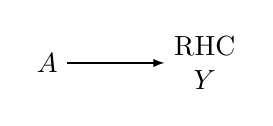
\begin{tikzpicture}
      \node (A) at (0,0) {$A$};
      \node[align=center] (Y) at (2,0) {RHC\checkmark\\$Y$};
      \draw[-latex] (A) -- (Y);
    \end{tikzpicture}
    \caption{Decision tree from treatment to outcome.}
  \end{figure}
\end{frame}

\begin{frame}{An adjacent diagram description}
  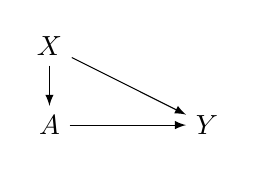
\begin{tikzpicture}
    \node (X) at (0,1) {$X$};
    \node (A) at (0,0) {$A$};
    \node (Y) at (2,0) {$Y$};
    \draw[-latex] (X) -- (A);
    \draw[-latex] (X) -- (Y);
    \draw[-latex] (A) -- (Y);
  \end{tikzpicture}
  \small{Causal DAG with observed treatment and outcome nodes}
\end{frame}

\end{document}
